% Chương 5
\chapter{Phân tích và thiết kế hệ thống}
\label{ch:chuong5}

\section{Các tác nhân hệ thống}
\begin{longtable}{|>{\raggedright\arraybackslash}p{0.095\dimexpr\linewidth-6\tabcolsep\relax}|>{\raggedright\arraybackslash}p{0.179\dimexpr\linewidth-6\tabcolsep\relax}|>{\raggedright\arraybackslash}p{0.726\dimexpr\linewidth-6\tabcolsep\relax}|}
\caption{Các tác nhân của hệ thống}\\
\hline
\textbf{STT} & \textbf{Tên tác nhân} & \textbf{Mô tả} \\ \hline
\endhead
1 & Người dùng & Là người dùng hệ thống đã được đăng ký tài khoản và đăng nhập vào ứng dụng có quyền quản lý tài khoản của mình và đăng xuất \\ \hline
2 & Bệnh nhân & Là người sử dụng hệ thống để hỗ trợ tiền chẩn đoán và trao đổi thông tin về bệnh da liễu.\newline Có thể hỏi đáp với chatbot, gửi hình ảnh và mô tả triệu chứng để hỗ trợ dự đoán bệnh.\newline Có thể tra cứu thông tin bệnh lý, các ca bệnh liên quan từ KB và đặt lịch khám với bác sĩ.\newline Có thể xem và quản lý hồ sơ bệnh án, lịch sử khám và các hình ảnh bệnh đã lưu trữ.\newline Có thể trao đổi trực tiếp với bác sĩ thông qua chat hoặc video call. Trong trường hợp bác sĩ chưa thể tiếp nhận, bệnh nhân có thể tiếp tục hỏi đáp với chatbot.\newline Thông tin từ cuộc trò chuyện với chatbot được hệ thống tổng hợp thành clinical fact và báo cáo hỗ trợ bác sĩ trước khi tư vấn. \\ \hline
3 & Bác sĩ & Là người sử dụng hệ thống để tiếp nhận, thăm khám, tư vấn và quản lý thông tin bệnh nhân.\newline Có thể xem báo cáo tổng hợp trước khi thực hiện thăm khám.\newline Có thể xem clinical fact, nguồn lập luận từ KB, lịch sử bệnh án và hồ sơ bệnh nhân.\newline Có thể chỉnh sửa, cập nhật hồ sơ sau mỗi lượt khám; lưu trữ ca bệnh và hình ảnh đã được xác nhận để làm dữ liệu tham khảo và phục vụ phát triển mô hình CNN.\newline Có thể trao đổi trực tiếp với bệnh nhân qua chat hoặc video call. Trong quá trình trao đổi, bác sĩ có thể xem các thông tin được chatbot tổng hợp và truy xuất tin nhắn nguồn làm bằng chứng cho từng kết luận.\newline Có thể trực quan hóa Knowledge Graph liên quan đến bệnh nhân.\newline Có thể tải lên giáo trình, guideline và tài liệu y khoa để bổ sung KB; phối hợp với chatbot để tra cứu và làm giàu KB. \\ \hline
\end{longtable}

\section{Usecase tổng quan}
\begin{figure}[H]
  \centering
  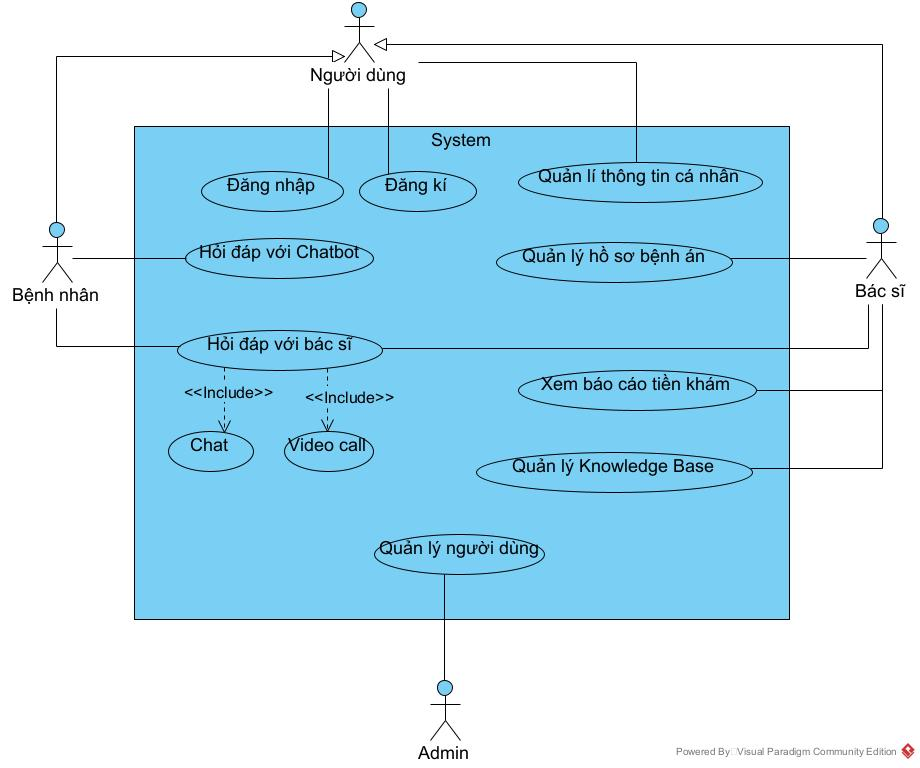
\includegraphics[width=0.95\linewidth,height=0.7\textheight,keepaspectratio]{chuong5/hinh/usecase_tong_quan.jpg}
  \caption{Sơ đồ usecase tổng quan của hệ thống}
\end{figure}

\subsection{Usecase Đăng ký (Sign Up)}
\begin{itemize}
  \item Cho phép người dùng mới tạo tài khoản trên hệ thống với vai trò tương ứng (bệnh nhân hoặc bác sĩ).
\end{itemize}

\subsection{Usecase Đăng nhập (Sign In)}
\begin{itemize}
  \item Xác thực danh tính người dùng để truy cập vào các chức năng tương ứng với quyền hạn của mình.
\end{itemize}

\subsection{Usecase Quản lý thông tin cá nhân (Profile Management)}
\begin{itemize}
  \item Cho phép xem, cập nhật và chỉnh sửa thông tin cá nhân, liên hệ, chuyên môn (đối với bác sĩ) hoặc thông tin cơ bản (đối với bệnh nhân).
\end{itemize}

\subsection{Usecase Hỏi đáp với Chatbot}
\begin{itemize}
  \item Bệnh nhân gửi mô tả triệu chứng và hình ảnh tổn thương da để nhận kết quả tiền chẩn đoán, giải thích ngắn gọn, dễ hiểu.
  \item Hệ thống tự động trích xuất các dữ kiện lâm sàng (\textit{clinical facts}) và tra cứu cơ sở tri thức (Knowledge Base - KB), ca bệnh tương tự để phục vụ tư vấn hoặc chuyển tiếp cho bác sĩ.
\end{itemize}

\subsection{Usecase Hỏi đáp với bác sĩ}
\begin{itemize}
  \item Cho phép bệnh nhân kết nối, tư vấn trực tiếp với bác sĩ khi cần thăm khám chuyên sâu. Gồm 2 chức năng thành phần:
  \begin{itemize}
    \item \textbf{Chat}: Nhắn tin trao đổi trực tiếp văn bản, hình ảnh.
    \item \textbf{Video call}: Thực hiện cuộc gọi video trực tuyến để bác sĩ quan sát rõ hơn tình trạng bệnh.
  \end{itemize}
  \item \textit{Lưu ý}: Trong khi chờ bác sĩ tiếp nhận, bệnh nhân tương tác với chatbot; nội dung này sẽ được tổng hợp lại cho bác sĩ trước khi trao đổi trực tiếp với bệnh nhân
\end{itemize}

\subsection{Usecase Xem báo cáo tiền khám}
\begin{itemize}
  \item Bác sĩ xem báo cáo tổng hợp tự động về bệnh nhân:
  \begin{itemize}
    \item Dựa trên các dữ kiện lâm sàng (\textit{clinical facts}) thu thập từ cuộc chat của bệnh nhân với chatbot.
    \item Hiển thị căn cứ/nguồn lập luận từ KB, biểu đồ tri thức (\textit{Knowledge Graph}) trực quan và lịch sử bệnh án liên quan.
  \end{itemize}
\end{itemize}

\subsection{Usecase Quản lý hồ sơ bệnh án}
\begin{itemize}
  \item Bác sĩ xem chi tiết hồ sơ bệnh nhân, lịch sử các lần khám.
  \item Bác sĩ cập nhật, chỉnh sửa kết luận chẩn đoán sau mỗi lượt khám; lưu trữ ca bệnh và hình ảnh làm chuẩn dữ liệu phục vụ tái huấn luyện mô hình đa CNN (\textit{multi-CNN}).
\end{itemize}

\subsection{Usecase Quản lý Knowledge Base (KB)}
\begin{itemize}
  \item Bác sĩ tải lên tài liệu y khoa, giáo trình chuyên ngành để làm giàu tri thức hệ thống.
  \item Tra cứu, kiểm duyệt và phối hợp cùng mô hình/chatbot để chuẩn hóa, mở rộng cơ sở tri thức da liễu phục vụ RAG.
\end{itemize}

\subsection{Quản lý người dùng}
\begin{itemize}
  \item Admin kiểm tra hồ sơ bác sĩ trước khi duyệt
\end{itemize}

\section{Thiết kế cơ sở dữ liệu}

\subsection{Thiết kế class}
\begin{figure}[H]
  \centering
  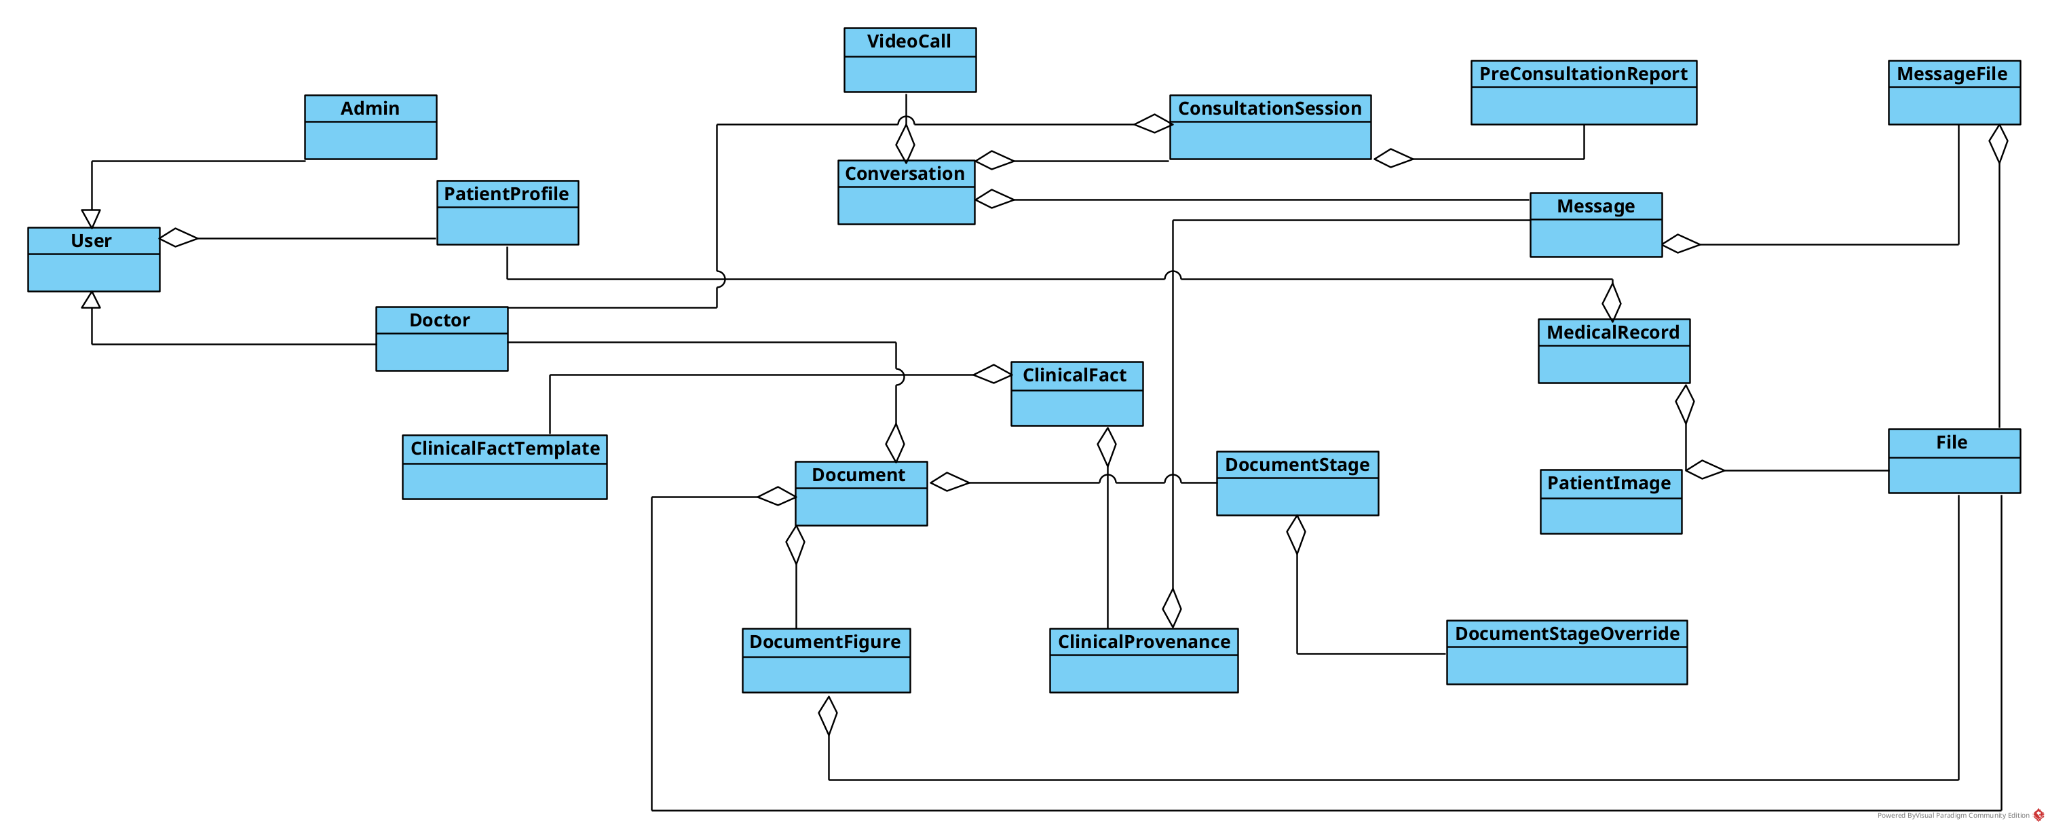
\includegraphics[width=0.95\linewidth,height=0.7\textheight,keepaspectratio]{chuong5/hinh/so_do_lop.png}
  \caption{Sơ đồ lớp của hệ thống}
\end{figure}

\subsection{Thiết kế CSDL}
\begin{figure}[H]
  \centering
  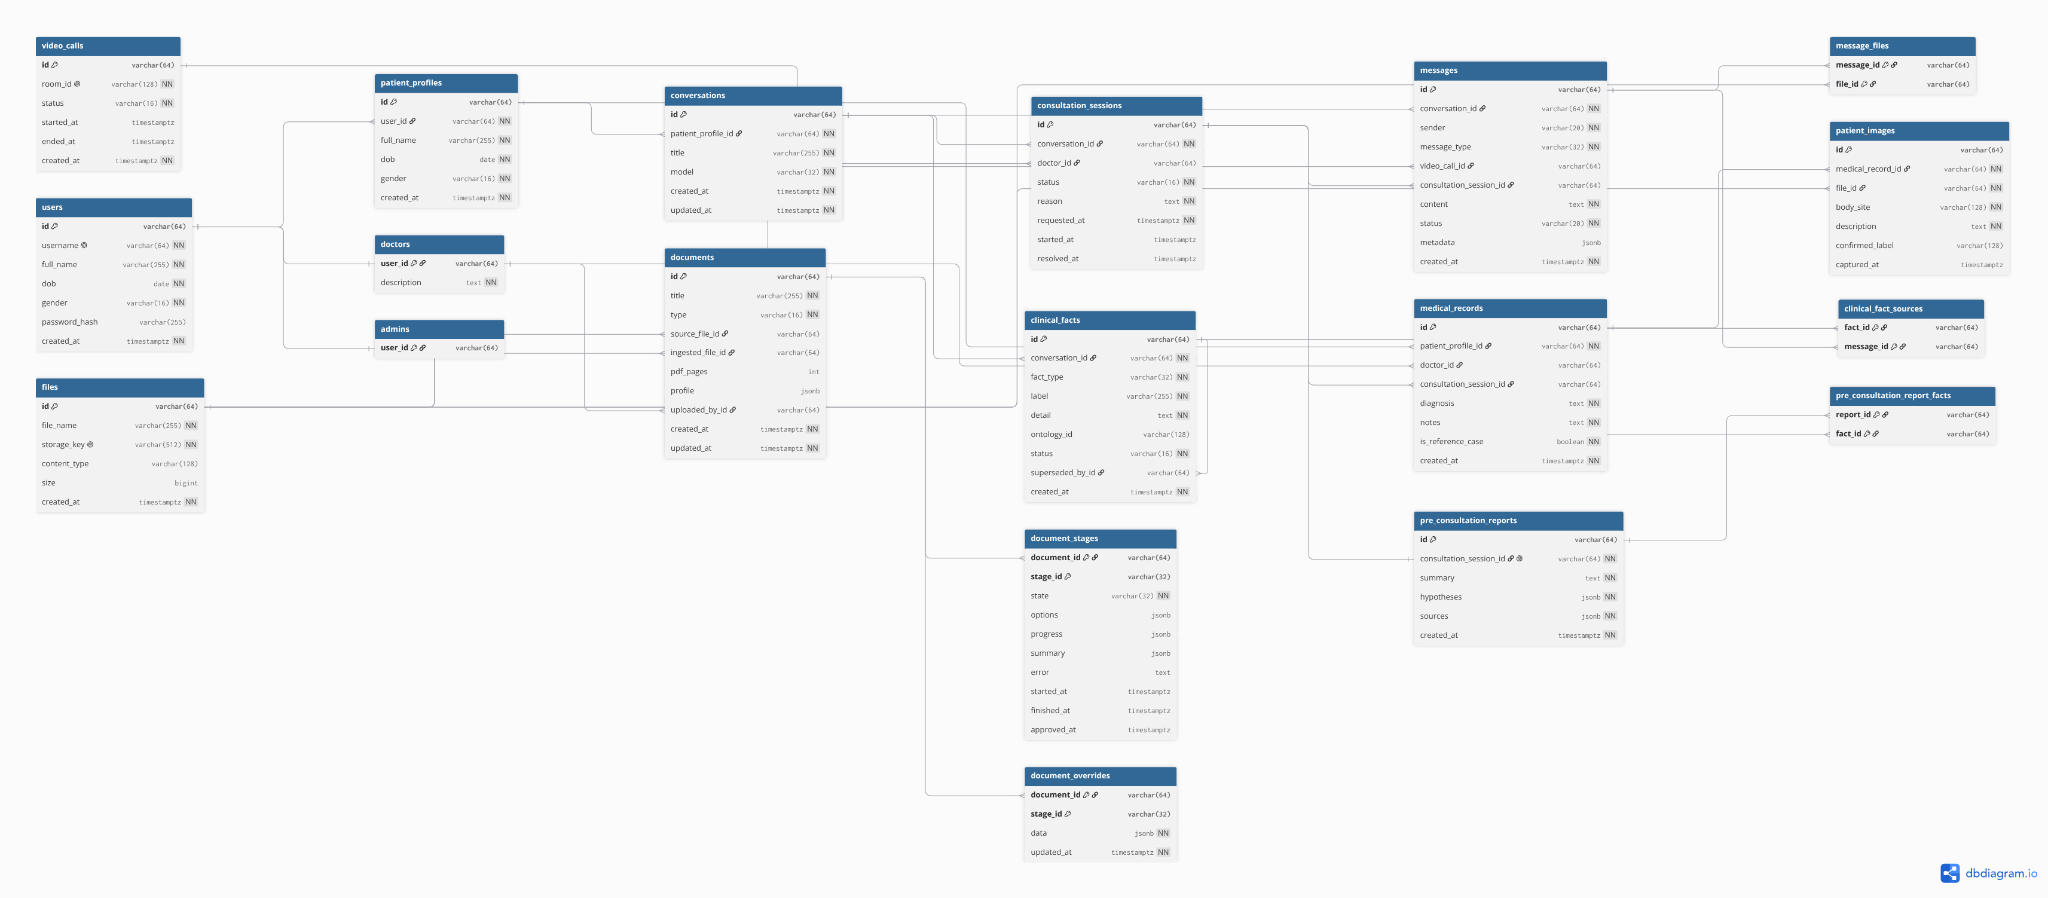
\includegraphics[width=0.95\linewidth,height=0.7\textheight,keepaspectratio]{chuong5/hinh/so_do_csdl.png}
  \caption{Sơ đồ cơ sở dữ liệu của hệ thống}
\end{figure}

\paragraph{Nhóm Người dùng}

\subparagraph{users -- tài khoản}

Field chung của mọi loại tài khoản. Vai trò bác sĩ / quản trị là bảng con 1-1 (doctors, admins), bệnh nhân là patient\_profiles. Chưa có API đăng ký / đăng nhập.
\begin{longtable}{|>{\raggedright\arraybackslash}p{0.250\dimexpr\linewidth-8\tabcolsep\relax}|>{\raggedright\arraybackslash}p{0.250\dimexpr\linewidth-8\tabcolsep\relax}|>{\raggedright\arraybackslash}p{0.250\dimexpr\linewidth-8\tabcolsep\relax}|>{\raggedright\arraybackslash}p{0.250\dimexpr\linewidth-8\tabcolsep\relax}|}
\hline
\textbf{Field} & \textbf{Kiểu} & \textbf{Null} & \textbf{Ý nghĩa} \\ \hline
\endhead
id & varchar(64) PK & không & Mã tài khoản, DB sinh. \\ \hline
username & varchar(64) & không, unique & Tên đăng nhập. \\ \hline
full\_name & varchar(255) & không & Họ tên đầy đủ. \\ \hline
dob & date & không & Ngày sinh. \\ \hline
gender & varchar(16) & không & male | female. \\ \hline
password\_hash & varchar(255) & có & Hash mật khẩu. NULL = tài khoản mẫu chưa đặt mật khẩu, chưa đăng nhập được. \\ \hline
created\_at & timestamptz & không & Thời điểm tạo tài khoản. \\ \hline
\end{longtable}

\subparagraph{patient\_profiles -- hồ sơ bệnh nhân}

Một tài khoản quản lý được nhiều hồ sơ (bản thân, người nhà). Hội thoại, bệnh án và dữ kiện lâm sàng đều gắn vào hồ sơ này, không gắn thẳng vào users.
\begin{longtable}{|>{\raggedright\arraybackslash}p{0.227\dimexpr\linewidth-8\tabcolsep\relax}|>{\raggedright\arraybackslash}p{0.273\dimexpr\linewidth-8\tabcolsep\relax}|>{\raggedright\arraybackslash}p{0.250\dimexpr\linewidth-8\tabcolsep\relax}|>{\raggedright\arraybackslash}p{0.250\dimexpr\linewidth-8\tabcolsep\relax}|}
\hline
\textbf{Field} & \textbf{Kiểu} & \textbf{Null} & \textbf{Ý nghĩa} \\ \hline
\endhead
id & varchar(64) PK & không & Mã hồ sơ. \\ \hline
user\_id & varchar(64) FK → users.id & không & Tài khoản quản lý hồ sơ. ON DELETE CASCADE. Có index. \\ \hline
full\_name & varchar(255) & không & Họ tên người bệnh (có thể khác chủ tài khoản). \\ \hline
dob & date & không & Ngày sinh người bệnh. \\ \hline
gender & varchar(16) & không & male | female. \\ \hline
created\_at & timestamptz & không & Thời điểm tạo hồ sơ. \\ \hline
\end{longtable}

\subparagraph{doctors -- vai trò bác sĩ}

Quan hệ 1-1 với users: PK đồng thời là FK nên một user chỉ có tối đa một dòng bác sĩ. Các bảng khác trỏ vào doctors.user\_id (không phải users.id) để DB chặn việc gán người không phải bác sĩ.
\begin{longtable}{|>{\raggedright\arraybackslash}p{0.250\dimexpr\linewidth-8\tabcolsep\relax}|>{\raggedright\arraybackslash}p{0.250\dimexpr\linewidth-8\tabcolsep\relax}|>{\raggedright\arraybackslash}p{0.250\dimexpr\linewidth-8\tabcolsep\relax}|>{\raggedright\arraybackslash}p{0.250\dimexpr\linewidth-8\tabcolsep\relax}|}
\hline
\textbf{Field} & \textbf{Kiểu} & \textbf{Null} & \textbf{Ý nghĩa} \\ \hline
\endhead
user\_id & varchar(64) PK, FK → users.id & không & Tài khoản được cấp vai trò bác sĩ. ON DELETE CASCADE. \\ \hline
description & text & không & Giới thiệu chuyên môn của bác sĩ. \\ \hline
\end{longtable}

\subparagraph{admins -- vai trò quản trị}

Quan hệ 1-1 với users, đánh dấu tài khoản quản trị (khu /admin/documents). Chưa có field riêng.
\begin{longtable}{|>{\raggedright\arraybackslash}p{0.250\dimexpr\linewidth-8\tabcolsep\relax}|>{\raggedright\arraybackslash}p{0.250\dimexpr\linewidth-8\tabcolsep\relax}|>{\raggedright\arraybackslash}p{0.250\dimexpr\linewidth-8\tabcolsep\relax}|>{\raggedright\arraybackslash}p{0.250\dimexpr\linewidth-8\tabcolsep\relax}|}
\hline
\textbf{Field} & \textbf{Kiểu} & \textbf{Null} & \textbf{Ý nghĩa} \\ \hline
\endhead
user\_id & varchar(64) PK, FK → users.id & không & Tài khoản quản trị. ON DELETE CASCADE. \\ \hline
\end{longtable}

\paragraph{Nhóm Hội thoại \& tư vấn}

\subparagraph{conversations -- cuộc hội thoại}

Một cuộc chat của một hồ sơ bệnh nhân. Chủ tài khoản suy ra qua patient\_profiles.user\_id, không lưu lặp ở đây.
\begin{longtable}{|>{\raggedright\arraybackslash}p{0.250\dimexpr\linewidth-8\tabcolsep\relax}|>{\raggedright\arraybackslash}p{0.228\dimexpr\linewidth-8\tabcolsep\relax}|>{\raggedright\arraybackslash}p{0.272\dimexpr\linewidth-8\tabcolsep\relax}|>{\raggedright\arraybackslash}p{0.250\dimexpr\linewidth-8\tabcolsep\relax}|}
\hline
\textbf{Field} & \textbf{Kiểu} & \textbf{Null} & \textbf{Ý nghĩa} \\ \hline
\endhead
id & varchar(64) PK & không & Mã hội thoại. \\ \hline
patient\_profile\_id & varchar(64) FK → patient\_profiles.id & không & Hồ sơ bệnh nhân sở hữu hội thoại. \\ \hline
title & varchar(255) & không, mặc định & Tiêu đề hiển thị trong danh sách chat. \\ \hline
model & varchar(32) & không & Id ngắn của model trong AGENT\_MODEL\_CHOICES (không phải chuỗi provider:model); worker tự map sang model thật khi chạy lượt, nên đổi danh sách model không cần migration. \\ \hline
created\_at & timestamptz & không & Thời điểm tạo. \\ \hline
updated\_at & timestamptz & không & Lần cập nhật gần nhất (tự cập nhật khi sửa). \\ \hline
\end{longtable}

\subparagraph{messages -- tin nhắn}

Một luồng chung cho AI, bệnh nhân và bác sĩ, phân biệt bằng sender. Các mốc tư vấn và cuộc gọi video cũng hiện thành tin trong luồng này.
\begin{longtable}{|>{\raggedright\arraybackslash}p{0.214\dimexpr\linewidth-8\tabcolsep\relax}|>{\raggedright\arraybackslash}p{0.230\dimexpr\linewidth-8\tabcolsep\relax}|>{\raggedright\arraybackslash}p{0.220\dimexpr\linewidth-8\tabcolsep\relax}|>{\raggedright\arraybackslash}p{0.336\dimexpr\linewidth-8\tabcolsep\relax}|}
\hline
\textbf{Field} & \textbf{Kiểu} & \textbf{Null} & \textbf{Ý nghĩa} \\ \hline
\endhead
id & varchar(64) PK & không & Mã tin nhắn. \\ \hline
conversation\_id & varchar(64) FK → conversations.id & không & Hội thoại chứa tin. \\ \hline
sender & varchar(20) & không & Người gửi: patient | ai | doctor. \\ \hline
message\_type & varchar(32) & không, mặc định text & Loại tin: text, attached (có đính kèm), video\_call, consultation\_requested, consultation\_accepted, consultation\_resolved. Là cột riêng để lọc / đếm theo loại. \\ \hline
video\_call\_id & varchar(64) FK → video\_calls.id & có & Chỉ điền với message\_type = video\_call. ON DELETE SET NULL. \\ \hline
consultation\_session\_id & varchar(64) FK → consultation\_sessions.id & có & Chỉ điền với 3 tin mốc consultation\_*: tin thuộc phiên tư vấn nào. ON DELETE SET NULL. Có index. \\ \hline
content & text & không, mặc định '' & Nội dung chữ. \\ \hline
status & varchar(20) & không & Trạng thái xử lý: queued | done | question (còn khai báo pending | streaming). question = agent đang chờ người dùng trả lời. \\ \hline
metadata & jsonb & có & Dữ liệu phụ (ORM đặt tên attribute là extra vì metadata trùng tên reserved của SQLAlchemy). Tin AI: reasoning[] (các bước lập luận), choice (câu hỏi lại), sources[] (nguồn trích dẫn). Tin người dùng: attached\_files, is\_option\_response. \\ \hline
created\_at & timestamptz & không & Thời điểm tạo tin. \\ \hline
\end{longtable}

\subparagraph{message\_files -- tệp đính kèm của tin nhắn (n-n)}

Bảng nối giữa tin nhắn và file. Một tin có thể đính kèm nhiều file, một file có thể được dùng lại ở nhiều chỗ.
\begin{longtable}{|>{\raggedright\arraybackslash}p{0.250\dimexpr\linewidth-8\tabcolsep\relax}|>{\raggedright\arraybackslash}p{0.250\dimexpr\linewidth-8\tabcolsep\relax}|>{\raggedright\arraybackslash}p{0.250\dimexpr\linewidth-8\tabcolsep\relax}|>{\raggedright\arraybackslash}p{0.250\dimexpr\linewidth-8\tabcolsep\relax}|}
\hline
\textbf{Field} & \textbf{Kiểu} & \textbf{Null} & \textbf{Ý nghĩa} \\ \hline
\endhead
message\_id & varchar(64) PK, FK → messages.id & không & Tin nhắn. ON DELETE CASCADE. \\ \hline
file\_id & varchar(64) PK, FK → files.id & không & File đính kèm. ON DELETE CASCADE. \\ \hline
\end{longtable}

\subparagraph{consultation\_sessions -- phiên tư vấn bác sĩ}

Mốc đánh dấu một lần bệnh nhân nhờ bác sĩ hỗ trợ; bảng này không chứa tin nhắn. Tin trao đổi nằm trong messages (sender = doctor), ba mốc yêu cầu / nhận / đóng là tin consultation\_* trỏ về phiên. Bác sĩ xem luồng chat từ đầu đến tin consultation\_resolved của phiên (phiên còn mở: tới hiện tại). Bệnh nhân vẫn chat AI song song. Mới có schema.
\begin{longtable}{|>{\raggedright\arraybackslash}p{0.250\dimexpr\linewidth-8\tabcolsep\relax}|>{\raggedright\arraybackslash}p{0.250\dimexpr\linewidth-8\tabcolsep\relax}|>{\raggedright\arraybackslash}p{0.250\dimexpr\linewidth-8\tabcolsep\relax}|>{\raggedright\arraybackslash}p{0.250\dimexpr\linewidth-8\tabcolsep\relax}|}
\hline
\textbf{Field} & \textbf{Kiểu} & \textbf{Null} & \textbf{Ý nghĩa} \\ \hline
\endhead
id & varchar(64) PK & không & Mã phiên. \\ \hline
conversation\_id & varchar(64) FK → conversations.id & không & Hội thoại có phiên tư vấn. ON DELETE CASCADE. Có index. \\ \hline
doctor\_id & varchar(64) FK → doctors.user\_id & có & Bác sĩ nhận ca. NULL khi chưa ai nhận. ON DELETE SET NULL. \\ \hline
status & varchar(16) & không, mặc định pending & pending (chờ bác sĩ nhận) → active (đang trao đổi) → resolved (đã đóng). \\ \hline
reason & text & không & Lý do bệnh nhân nhờ bác sĩ. \\ \hline
requested\_at & timestamptz & không & Lúc bệnh nhân gửi yêu cầu. \\ \hline
started\_at & timestamptz & có & Lúc bác sĩ nhận. \\ \hline
resolved\_at & timestamptz & có & Lúc đóng phiên. \\ \hline
\end{longtable}

Ràng buộc:
\begin{itemize}
  \item CHECK doctor\_when\_not\_pending: status = 'pending' OR doctor\_id IS NOT NULL --- phiên đã nhận hoặc đã đóng thì bắt buộc có bác sĩ.
  \item CHECK resolved\_at\_when\_resolved: status <> 'resolved' OR resolved\_at IS NOT NULL.
  \item Unique một phần uq\_consultation\_sessions\_open\_per\_conversation trên conversation\_id với điều kiện status <> 'resolved' --- mỗi hội thoại tối đa 1 phiên đang mở, vì tin bác sĩ gắn với phiên theo khoảng thời gian, hai phiên mở cùng lúc sẽ không phân biệt được.
\end{itemize}

\subparagraph{video\_calls -- cuộc gọi video}

Tách bảng riêng (không chỉ nằm trong messages.metadata) vì cuộc gọi có vòng đời pending → ongoing → ended được cập nhật sau khi tin nhắn đã tạo. Tin message\_type = video\_call trỏ tới đây qua messages.video\_call\_id. Mới có schema.
\begin{longtable}{|>{\raggedright\arraybackslash}p{0.250\dimexpr\linewidth-8\tabcolsep\relax}|>{\raggedright\arraybackslash}p{0.250\dimexpr\linewidth-8\tabcolsep\relax}|>{\raggedright\arraybackslash}p{0.250\dimexpr\linewidth-8\tabcolsep\relax}|>{\raggedright\arraybackslash}p{0.250\dimexpr\linewidth-8\tabcolsep\relax}|}
\hline
\textbf{Field} & \textbf{Kiểu} & \textbf{Null} & \textbf{Ý nghĩa} \\ \hline
\endhead
id & varchar(64) PK & không & Mã cuộc gọi. \\ \hline
room\_id & varchar(128) & không, unique & Mã phòng video. \\ \hline
status & varchar(16) & không, mặc định pending & pending | ongoing | ended. \\ \hline
started\_at & timestamptz & có & Lúc bắt đầu gọi. \\ \hline
ended\_at & timestamptz & có & Lúc kết thúc. \\ \hline
created\_at & timestamptz & không & Lúc tạo cuộc gọi. \\ \hline
\end{longtable}

\paragraph{Nhóm Bệnh án}

\subparagraph{medical\_records -- bệnh án}

Bệnh án do bác sĩ ghi cho một hồ sơ bệnh nhân; một hồ sơ có nhiều bệnh án. Không gắn với phiên tư vấn cụ thể. Mới có schema.
\begin{longtable}{|>{\raggedright\arraybackslash}p{0.250\dimexpr\linewidth-8\tabcolsep\relax}|>{\raggedright\arraybackslash}p{0.250\dimexpr\linewidth-8\tabcolsep\relax}|>{\raggedright\arraybackslash}p{0.250\dimexpr\linewidth-8\tabcolsep\relax}|>{\raggedright\arraybackslash}p{0.250\dimexpr\linewidth-8\tabcolsep\relax}|}
\hline
\textbf{Field} & \textbf{Kiểu} & \textbf{Null} & \textbf{Ý nghĩa} \\ \hline
\endhead
id & varchar(64) PK & không & Mã bệnh án. \\ \hline
patient\_profile\_id & varchar(64) FK → patient\_profiles.id & không & Hồ sơ bệnh nhân. ON DELETE CASCADE. Có index. \\ \hline
doctor\_id & varchar(64) FK → doctors.user\_id & có & Bác sĩ ghi bệnh án. ON DELETE SET NULL --- bác sĩ bị xoá thì bệnh án vẫn giữ. \\ \hline
diagnosis & text & không & Chẩn đoán của bác sĩ. \\ \hline
notes & text & không, mặc định '' & Ghi chú thêm. \\ \hline
is\_reference\_case & boolean & không, mặc định false & Ca bệnh tham khảo: bác sĩ xác nhận dùng làm dữ liệu cho KB / chatbot tra ca tương tự (phải ẩn định danh khi đưa vào KB). \\ \hline
created\_at & timestamptz & không & Lúc ghi bệnh án. \\ \hline
\end{longtable}

\subparagraph{patient\_images -- ảnh bệnh}

Ảnh bệnh do bác sĩ gắn vào bệnh án. Trỏ FK tới files thay vì chép file, nên bác sĩ chọn lại được ảnh bệnh nhân đã gửi trong chat mà không tạo bản sao trong MinIO. Mới có schema.
\begin{longtable}{|>{\raggedright\arraybackslash}p{0.250\dimexpr\linewidth-8\tabcolsep\relax}|>{\raggedright\arraybackslash}p{0.250\dimexpr\linewidth-8\tabcolsep\relax}|>{\raggedright\arraybackslash}p{0.250\dimexpr\linewidth-8\tabcolsep\relax}|>{\raggedright\arraybackslash}p{0.250\dimexpr\linewidth-8\tabcolsep\relax}|}
\hline
\textbf{Field} & \textbf{Kiểu} & \textbf{Null} & \textbf{Ý nghĩa} \\ \hline
\endhead
id & varchar(64) PK & không & Mã ảnh. \\ \hline
medical\_record\_id & varchar(64) FK → medical\_records.id & không & Bệnh án chứa ảnh. ON DELETE CASCADE. Có index. \\ \hline
file\_id & varchar(64) FK → files.id & không & File ảnh trong MinIO. ON DELETE CASCADE. \\ \hline
body\_site & varchar(128) & không, mặc định '' & Vị trí trên cơ thể. \\ \hline
description & text & không, mặc định '' & Mô tả tổn thương. \\ \hline
confirmed\_label & varchar(128) & có & Nhãn bác sĩ xác nhận, nên khớp tên lớp của CNN để dùng làm dữ liệu huấn luyện. \\ \hline
captured\_at & timestamptz & có & Thời điểm chụp ảnh. \\ \hline
\end{longtable}

\paragraph{Nhóm Lâm sàng}

Luồng ý tưởng: agent trích dữ kiện lâm sàng từ hội thoại, mỗi dữ kiện luôn tạo từ một mẫu chuẩn, ghi lại tin nhắn nguồn, và khi bệnh nhân nhờ bác sĩ thì có một báo cáo tóm tắt cho phiên đó. Cả nhóm mới có schema, chưa có bước trích xuất.

\subparagraph{clinical\_fact\_templates -- mẫu dữ kiện lâm sàng}

Danh mục chuẩn (ví dụ "ngứa", "dị ứng penicillin"). Agent chỉ được trích fact theo mẫu có sẵn để nhãn và ontology\_id nhất quán giữa các bệnh nhân.
\begin{longtable}{|>{\raggedright\arraybackslash}p{0.250\dimexpr\linewidth-8\tabcolsep\relax}|>{\raggedright\arraybackslash}p{0.250\dimexpr\linewidth-8\tabcolsep\relax}|>{\raggedright\arraybackslash}p{0.250\dimexpr\linewidth-8\tabcolsep\relax}|>{\raggedright\arraybackslash}p{0.250\dimexpr\linewidth-8\tabcolsep\relax}|}
\hline
\textbf{Field} & \textbf{Kiểu} & \textbf{Null} & \textbf{Ý nghĩa} \\ \hline
\endhead
id & varchar(64) PK & không & Mã mẫu. \\ \hline
fact\_type & varchar(32) & không & Loại: symptom (triệu chứng cơ năng), lesion (tổn thương da), history (tiền sử / diễn tiến), medication (thuốc), allergy (dị ứng), image\_finding (kết quả phân loại ảnh, chỉ là giả thuyết), other. \\ \hline
label & varchar(255) & không, unique & Tên chuẩn của mẫu. \\ \hline
description & text & không, mặc định '' & Gợi ý cho agent / bác sĩ biết cần hỏi và ghi gì vào clinical\_facts.detail. \\ \hline
ontology\_id & varchar(128) & có & Id DermO / PrimeKG đã chuẩn hoá, dùng để vẽ KG liên quan bệnh nhân. \\ \hline
\end{longtable}

\subparagraph{clinical\_facts -- dữ kiện lâm sàng}

Dữ kiện của hồ sơ bệnh nhân (không thuộc riêng một cuộc chat), luôn tạo từ một mẫu. Không sửa đè: bệnh nhân đính chính thì tạo fact mới và đánh dấu fact cũ superseded, để bác sĩ vẫn thấy lịch sử khai báo. Hội thoại sinh ra fact truy ngược qua clinical\_provenances → messages.
\begin{longtable}{|>{\raggedright\arraybackslash}p{0.250\dimexpr\linewidth-8\tabcolsep\relax}|>{\raggedright\arraybackslash}p{0.250\dimexpr\linewidth-8\tabcolsep\relax}|>{\raggedright\arraybackslash}p{0.250\dimexpr\linewidth-8\tabcolsep\relax}|>{\raggedright\arraybackslash}p{0.250\dimexpr\linewidth-8\tabcolsep\relax}|}
\hline
\textbf{Field} & \textbf{Kiểu} & \textbf{Null} & \textbf{Ý nghĩa} \\ \hline
\endhead
id & varchar(64) PK & không & Mã fact. \\ \hline
patient\_profile\_id & varchar(64) FK → patient\_profiles.id & không & Hồ sơ bệnh nhân sở hữu fact. ON DELETE CASCADE. Có index. \\ \hline
template\_id & varchar(64) FK → clinical\_fact\_templates.id & không & Mẫu của fact; loại / nhãn / ontology lấy từ mẫu. ON DELETE RESTRICT --- không xoá được mẫu đang có fact dùng. Có index. \\ \hline
detail & text & không, mặc định '' & Giá trị cụ thể của bệnh nhân: vị trí, thời gian khởi phát, mức độ, diễn tiến... \\ \hline
status & varchar(16) & không, mặc định active & active | superseded (đã bị fact mới thay). \\ \hline
superseded\_by\_id & varchar(64) FK → clinical\_facts.id (tự tham chiếu) & có & Fact mới thay thế fact này. ON DELETE SET NULL. \\ \hline
created\_at & timestamptz & không & Lúc ghi fact. \\ \hline
\end{longtable}

\subparagraph{clinical\_provenances -- nguồn gốc của fact (n-n)}

Bảng nối giữa fact và tin nhắn, thể hiện entity ClinicalProvenance. Một fact có

thể đến từ nhiều tin (kể cả ở nhiều hội thoại), một tin có thể sinh nhiều fact. Fact do bác sĩ tự nhập thì không có dòng nào ở đây. Sau này muốn thêm thông tin riêng cho mỗi cặp (đoạn trích, độ tin cậy) thì thêm cột vào bảng này.
\begin{longtable}{|>{\raggedright\arraybackslash}p{0.250\dimexpr\linewidth-8\tabcolsep\relax}|>{\raggedright\arraybackslash}p{0.250\dimexpr\linewidth-8\tabcolsep\relax}|>{\raggedright\arraybackslash}p{0.250\dimexpr\linewidth-8\tabcolsep\relax}|>{\raggedright\arraybackslash}p{0.250\dimexpr\linewidth-8\tabcolsep\relax}|}
\hline
\textbf{Field} & \textbf{Kiểu} & \textbf{Null} & \textbf{Ý nghĩa} \\ \hline
\endhead
fact\_id & varchar(64) PK, FK → clinical\_facts.id & không & Fact. ON DELETE CASCADE. \\ \hline
message\_id & varchar(64) PK, FK → messages.id & không & Tin nhắn gốc làm bằng chứng. ON DELETE CASCADE. \\ \hline
\end{longtable}

\subparagraph{pre\_consultation\_reports -- báo cáo tiền tư vấn}

Báo cáo AI tóm tắt cho bác sĩ đọc trước khi nhận ca, 1 báo cáo / phiên tư vấn. Chỉ là gợi ý hỗ trợ, không phải chẩn đoán y khoa. Tạm thời chỉ có phần tóm tắt; fact lâm sàng bác sĩ xem trực tiếp từ hồ sơ bệnh nhân.
\begin{longtable}{|>{\raggedright\arraybackslash}p{0.250\dimexpr\linewidth-8\tabcolsep\relax}|>{\raggedright\arraybackslash}p{0.250\dimexpr\linewidth-8\tabcolsep\relax}|>{\raggedright\arraybackslash}p{0.250\dimexpr\linewidth-8\tabcolsep\relax}|>{\raggedright\arraybackslash}p{0.250\dimexpr\linewidth-8\tabcolsep\relax}|}
\hline
\textbf{Field} & \textbf{Kiểu} & \textbf{Null} & \textbf{Ý nghĩa} \\ \hline
\endhead
id & varchar(64) PK & không & Mã báo cáo. \\ \hline
consultation\_session\_id & varchar(64) FK → consultation\_sessions.id & không, unique & Phiên tư vấn của báo cáo; unique tạo quan hệ 1-1. ON DELETE CASCADE. \\ \hline
summary & text & không & Nội dung tóm tắt. \\ \hline
created\_at & timestamptz & không & Lúc sinh báo cáo. \\ \hline
\end{longtable}

\paragraph{Nhóm File}

\subparagraph{files -- metadata file trong MinIO}

Dùng chung cho ảnh đính kèm tin nhắn, ảnh bệnh trong bệnh án và file của tài liệu. Nội dung file nằm ở MinIO, không nằm trong DB.
\begin{longtable}{|>{\raggedright\arraybackslash}p{0.250\dimexpr\linewidth-8\tabcolsep\relax}|>{\raggedright\arraybackslash}p{0.250\dimexpr\linewidth-8\tabcolsep\relax}|>{\raggedright\arraybackslash}p{0.250\dimexpr\linewidth-8\tabcolsep\relax}|>{\raggedright\arraybackslash}p{0.250\dimexpr\linewidth-8\tabcolsep\relax}|}
\hline
\textbf{Field} & \textbf{Kiểu} & \textbf{Null} & \textbf{Ý nghĩa} \\ \hline
\endhead
id & varchar(64) PK & không & Mã file. \\ \hline
file\_name & varchar(255) & không & Tên hiển thị (ví dụ tên file gốc người dùng upload). \\ \hline
storage\_key & varchar(512) & không, unique & Khoá đầy đủ của object trong bucket MinIO (không phải đường dẫn tương đối trong thư mục của entity). \\ \hline
content\_type & varchar(128) & có & MIME type, ví dụ application/pdf. \\ \hline
size & bigint & có & Dung lượng, đơn vị byte. \\ \hline
created\_at & timestamptz & không & Lúc tạo bản ghi. \\ \hline
\end{longtable}

\paragraph{Nhóm Tài liệu (pipeline số hoá sách)}

Admin upload PDF → qua 4 bước (ingest → toc → chunks → index), mỗi bước người duyệt phải approve trước khi bước sau chạy. Entity lồng nhau: Document → DocumentStage → DocumentStageOverride.

\subparagraph{documents -- tài liệu}
\begin{longtable}{|>{\raggedright\arraybackslash}p{0.250\dimexpr\linewidth-8\tabcolsep\relax}|>{\raggedright\arraybackslash}p{0.250\dimexpr\linewidth-8\tabcolsep\relax}|>{\raggedright\arraybackslash}p{0.250\dimexpr\linewidth-8\tabcolsep\relax}|>{\raggedright\arraybackslash}p{0.250\dimexpr\linewidth-8\tabcolsep\relax}|}
\hline
\textbf{Field} & \textbf{Kiểu} & \textbf{Null} & \textbf{Ý nghĩa} \\ \hline
\endhead
id & varchar(64) PK & không & Mã tài liệu; cũng là tên thư mục document/<id>/ trong MinIO và document\_id trong payload Qdrant. \\ \hline
title & varchar(255) & không & Tiêu đề. \\ \hline
type & varchar(16) & không, mặc định book & book | image | video | other. Hiện chỉ book đi qua pipeline. \\ \hline
source\_file\_id & varchar(64) FK → files.id & có & File gốc người dùng upload (source.pdf). ON DELETE SET NULL. \\ \hline
ingested\_file\_id & varchar(64) FK → files.id & có & Kết quả bước ingest (pages.jsonl); chỉ có khi đã qua bước ingest. ON DELETE SET NULL. \\ \hline
pdf\_pages & int & có & Số trang PDF; chỉ có với type = book. \\ \hline
profile & jsonb & có & Cấu hình xử lý của tài liệu (engine đọc chữ, tham số...), đọc / ghi qua Pydantic (app/models/document\_profile.py::Profile). \\ \hline
uploaded\_by\_id & varchar(64) FK → doctors.user\_id & có & Bác sĩ tải lên (chỉ bác sĩ được tải). ON DELETE SET NULL; NULL với tài liệu tạo trước khi có đăng nhập. \\ \hline
created\_at & timestamptz & không & Lúc tạo. \\ \hline
updated\_at & timestamptz & không & Lần cập nhật gần nhất (tự cập nhật). \\ \hline
\end{longtable}

\subparagraph{document\_stages -- trạng thái từng bước}

4 dòng cho mỗi tài liệu (ingest, toc, chunks, index), tạo cùng lúc với tài liệu. Có khoá id riêng để document\_overrides trỏ tới mà không phải lặp document\_id.
\begin{longtable}{|>{\raggedright\arraybackslash}p{0.250\dimexpr\linewidth-8\tabcolsep\relax}|>{\raggedright\arraybackslash}p{0.250\dimexpr\linewidth-8\tabcolsep\relax}|>{\raggedright\arraybackslash}p{0.250\dimexpr\linewidth-8\tabcolsep\relax}|>{\raggedright\arraybackslash}p{0.250\dimexpr\linewidth-8\tabcolsep\relax}|}
\hline
\textbf{Field} & \textbf{Kiểu} & \textbf{Null} & \textbf{Ý nghĩa} \\ \hline
\endhead
id & varchar(64) PK & không & Mã dòng bước. \\ \hline
document\_id & varchar(64) FK → documents.id & không & Tài liệu. ON DELETE CASCADE. \\ \hline
stage\_id & varchar(32) & không & Mã bước: ingest | toc | chunks | index. Cặp (document\_id, stage\_id) là unique. \\ \hline
state & varchar(32) & không, mặc định not\_started & not\_started → running → pending\_review → approved; ngoài ra failed, cancelled, và stale (bước phía trước chạy lại nên kết quả cũ không còn đúng). \\ \hline
options & jsonb & có & Tham số của lần chạy. \\ \hline
progress & jsonb & có & Tiến độ khi đang chạy (FE poll để hiển thị). \\ \hline
summary & jsonb & có & Tóm tắt kết quả, hiển thị cho người duyệt. \\ \hline
error & text & có & Thông báo lỗi khi failed; lỗi người dùng sửa được hiển thị nguyên văn trên UI. \\ \hline
started\_at & timestamptz & có & Lúc bắt đầu chạy. \\ \hline
finished\_at & timestamptz & có & Lúc chạy xong / dừng. \\ \hline
approved\_at & timestamptz & có & Lúc người duyệt approve. \\ \hline
\end{longtable}

\subparagraph{document\_overrides -- sửa tay của người duyệt}

Chỉnh sửa tay của người duyệt lên kết quả một bước, tách khỏi kết quả máy để chạy lại bước không mất công sửa. Thuộc về bước qua document\_stage\_id, tài liệu suy ra từ bước đó. Hiện tối đa 1 dòng / bước.
\begin{longtable}{|>{\raggedright\arraybackslash}p{0.250\dimexpr\linewidth-8\tabcolsep\relax}|>{\raggedright\arraybackslash}p{0.250\dimexpr\linewidth-8\tabcolsep\relax}|>{\raggedright\arraybackslash}p{0.250\dimexpr\linewidth-8\tabcolsep\relax}|>{\raggedright\arraybackslash}p{0.250\dimexpr\linewidth-8\tabcolsep\relax}|}
\hline
\textbf{Field} & \textbf{Kiểu} & \textbf{Null} & \textbf{Ý nghĩa} \\ \hline
\endhead
document\_stage\_id & varchar(64) PK, FK → document\_stages.id & không & Bước được sửa. ON DELETE CASCADE. \\ \hline
data & jsonb & không, mặc định \{\} & Nội dung sửa tay. Ví dụ bước toc: \{<id mục>: \{...\}, \_deleted, \_added, \_offset\} (sửa mục, xoá, thêm, lệch số trang). Giá trị null khi cập nhật nghĩa là hoàn tác một override. \\ \hline
updated\_at & timestamptz & không & Lần sửa gần nhất (tự cập nhật). \\ \hline
\end{longtable}

\section{Kết luận chương}

Chương này đã phân tích và thiết kế hệ thống. Hệ thống có ba tác nhân chính là người dùng, bệnh nhân và bác sĩ, với các usecase từ đăng ký, đăng nhập, quản lý thông tin cá nhân, hỏi đáp với chatbot, tư vấn trực tiếp với bác sĩ, xem báo cáo tiền khám, quản lý hồ sơ bệnh án đến quản lý cơ sở tri thức. Cơ sở dữ liệu được thiết kế theo các nhóm: người dùng, hội thoại và tư vấn, bệnh án, dữ kiện lâm sàng, tệp và tài liệu, bảo đảm lưu vết nguồn gốc của dữ kiện từ tin nhắn tới báo cáo.

Thiết kế này là cơ sở cho việc cài đặt và triển khai hệ thống ở chương sau.
